% LaTeX file for a 1 page document
\documentclass[12pt]{report}
\usepackage{amsmath}
\usepackage{amssymb}
\usepackage{amsthm}
%\usepackage{physymb}
\usepackage{graphicx}
%\usepackage{wrapfig}
\bibliographystyle{plain}
\usepackage{tikz}
\usepackage{natbib}
\usetikzlibrary{calc,patterns,decorations.pathmorphing,decorations.markings}

\title{Simulation of an Orrery in Box2D\\ A CS296 Report by Group 07}
\author{Ranveer Aggarwal (120050020) \\ ranveeraggarwal@gmail.com \and Devdeep Ray (120050007) \\ devdeep.ray1994@iitb.ac.in \and Sasibhushan Rallabandi (120050056) \\ sasiralla@iitb.ac.in}
\date{}

\begin{document}
\maketitle

\chapter*{Introduction}
An orrery is a mechanical model of the solar system device that illustrates the relative sizes, positions, and motions of the planets and moons according to the heliocentric model.

\begin{center}
\setlength\fboxsep{2pt}
\setlength\fboxrule{1pt}
\fbox{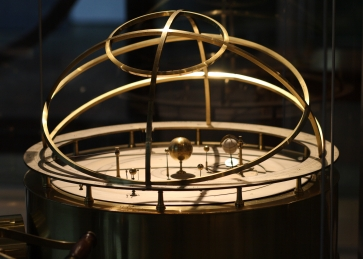
\includegraphics[scale=0.1]{./img/orrery-main.jpg}}
\end{center}

Though the Greeks had working planetaria, the first orrery that was a planetarium of the modern era was produced in 1704, and one was presented to the Earl of Orrery — whence came the name. They are typically driven by a clockwork mechanism with a globe representing the Sun at the centre, and with a planet at the end of each of the arms.


\pagebreak

\chapter*{Physics behind the simulation}

\begin{center}
\setlength\fboxsep{2pt}
\setlength\fboxrule{1pt}
\fbox{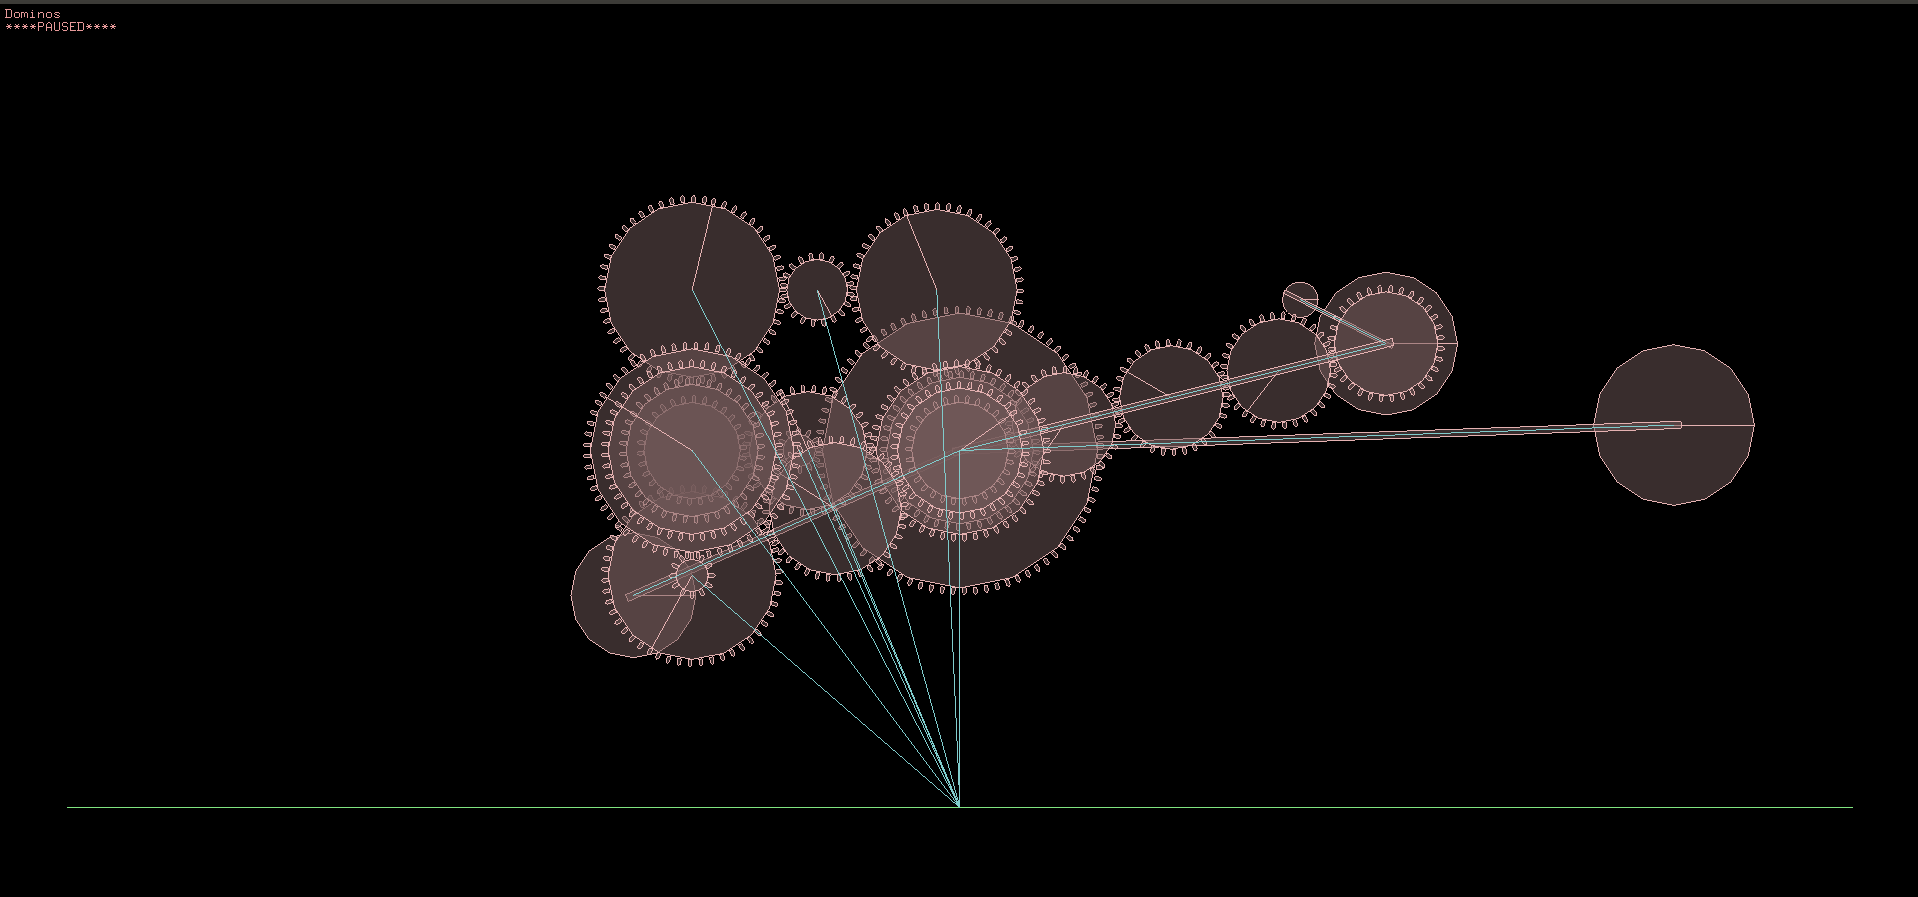
\includegraphics[scale=0.2]{./img/gui.png}}
\end{center}

\pagebreak
\bibliography{report}

\end{document}
}
